\chapter{Vývojová dokumentace}
V~této kapitole se budeme detailněji věnovat implementaci našeho řešení. Rozebereme její strukturu, jednotlivé části programu a~rozhodnutí, která bylo potřeba učinit. Po přečtení kapitoly by měl být čtenář schopen orientovat se v~našem řešení a~rozumět účelu jeho jednotlivých částí. Podrobně též popíšeme zapojení řešiče do infrastruktury OpenSMT.

Vzhledem k~povaze řešení jakožto interní součásti většího frameworku neobsahuje tato práce uživatelskou dokumentaci. Návod na spuštění OpenSMT a~názornou ukázku jeho použití na problému využívajícím náš řešič nalezneme v~přílohách \ref{content}~a~\ref{priklad}.
\section{Datové struktury}\label{data}

\subsection*{Struktury OpenSMT}
Základní datovou strukturou v~OpenSMT je \icode{Pterm}, reprezentující jeden term vyskytující se ve vstupní formuli. Odkazy na tyto termy jsou pak předávány pomocí referenční struktury \icode{PTRef}. Ta obsahuje pouze numerický identifikátor použitý k~jejímu rozlišení. Mapování jednotlivých referencí na odpovídající termy přitom zařizuje třída \icode{Logic}, respektive její potomci. \icode{Logic} si ukládá převodní tabulku párující \icode{PTRef} a~jejich odpovídající \icode{Pterm} a~poskytuje také mechanismy pro vytváření nových termů. Její potomci pak rozšiřují tyto mechanismy o~možnosti odpovídající dané teorii, např. s~\icode{LALogic} jsme schopni vytvářet termy odpovídající nerovnicím z~lineární aritmetiky. Jelikož rozdílová omezení jsou speficickým tvarem lineárních nerovnic, využívá náš řešič právě schopností \icode{LALogic}, konkrétně \icode{LIALogic} pro implementovanou celočíselnou verzi.

Ohodnocení proměnných je uloženo ve struktuře \icode{PtAsgn}, která obsahuje \icode{PTRef} odpovídající ohodnocené proměnné a~\icode{lbool} označující její ohodnocení (\icode{lbool} je běžný optional boolean).

Samotné termy mají stromovou strukturu. Pokud se nejedná o~atomickou proměnnou, reprezentuje term nějaký $n$-ární funkční či relační symbol společně s~jeho argumenty. K~rozlišení typu symbolu nám opět poslouží API třídy \icode{Logic}, pro přístup k~argumentům je pak použit operátor \icode{[]}. Reprezentuje-li například \icode{Pterm~p} term $(x \lor y)$, budeme mít přístup k~proměnným \icode{p[0]} a~\icode{p[1]}, což jsou \icode{PTRef} reprezentující $x$, respektive $y$. 

\begin{code}[label=Příklad práce s~termem p $\approx (4 \leq x)$]
PTRef p;    
assert( logic.isNumLeq(p) );
Pterm &term = logic.getPterm(p);

PTRef c = term[0];
assert( logic.isNumConst(c) );
opensmt::Number n = logic.getNumConst(c);
assert( n == 4 );

PTRef x = term[1];
assert( logic.isNumVar(x) );
\end{code}

Je vhodné zmínit, že za dobu vývoje OpenSMT v~něm vzniklo několik implementací základních datových struktur. Hojně užívaným příkladem je třída \icode{vec}, reprezentující běžný vektor. Vyjma malých rozdílů API a~údajné vyšší efektivity na primitivních typech se tyto třídy výrazně neliší od implementací ze standardní knihovny. Konkrétně třída \icode{vec} je navíc omezena skutečností, že jejími prvky nemohou být typy obsahující odkazy (vyjímkou z~tohoto pravidla je zvlášť implementovaný \icode{vec$\langle$vec$\langle$T$\rangle\rangle$}). Za účelem konzistence se zbytkem frameworku jsme se přesto rozhodli využívat tyto lokální implementace struktur všude, kde je to možné. 

\subsection*{Struktury řešiče}
Nejdůležitější datovou strukturou našeho řešiče je \icode{Edge}. V~té jsou uloženy informace o~jedné hraně omezujícího grafu. Konkrétně tedy obsahuje reference na její vstupní a~výstupní vrchol, ohodnocení, odkaz na svou negaci a~informaci o~tom, kdy byla přidána do omezujícího grafu. Po vzoru frameworku přitom zbytek řešiče nepracuje přímo s~těmito strukturami, ale s~jejich referencemi \icode{EdgeRef}, které opět obsahují pouze jednoznačný numerický identifikátor. Samotné hrany se pak nacházejí jen v~centrálním úložišti, které tvoří třída \icode{STPStore}. Ta zařizuje zejména tvorbu nových hran a~převod z~\icode{EdgeRef} na \icode{Edge\&}. Použit je i~protějšek k~\icode{EdgeRef} pro vrcholy, struktura \icode{VertexRef}. Jelikož se však s~vrcholy nepojí žádná informace, nejedná se o~odkaz na další strukturu, ale pouze o~symbolické reference, sloužící pro vzájemné rozlišení jednotlivých vrcholů.

%\captionof{verbatim}{test}
\begin{code}[label=Deklarace struktury Edge]
struct Edge {
    VertexRef from, to;    
    EdgeRef neg;           
    ptrdiff_t cost;
    uint32_t setTime;
}
\end{code}

Jelikož náš řešič dostává od frameworku informace o~proměnných zásadně jako \icode{PTRef}, potřebujeme způsob, jak přecházet mezi reprezentací frameworku a~interní reprezentací našeho řešiče. K~tomuto účelu slouží třída \icode{STPMapper}. V~této třídě se vyskytuje hned několik druhů převodních tabulek. Pamatuje si převod z~\icode{PTRef} na \icode{VertexRef}, přiřazující proměnné k~vrcholům grafu, a~převod z~\icode{PTRef} na \icode{EdgeRef}, přiřazující nerovnice k~hranám. Tyto převody jsou zásadní pro interpretaci příkazů frameworku. Pro hrany si pamatuje i~opačný převod, mapující \icode{EdgeRef} zpět na odpovídající \icode{PTRef}. Ten je důležitý pro oznámení nalezených dedukcí (viz.~\ref{dusl}). Pro účely oznámení nesplnitelné množiny literálů si pro hrany právě v~grafu pamatujeme i~mapu z~\icode{EdgeRef} na \icode{PtAsgn}, které způsobily jejich přidání do grafu. Uvědomme si, že tento převod není zaměnitelný s~předchozím převodem na \icode{PTRef}, jelikož hrana se může vyskytnout v~grafu z~důvodu záporného ohodnocení její negace. \icode{STPMapper} si navíc pamatuje pro každý vrchol seznam všech hran, ve kterých se daný vrchol vyskytuje, jak je popsáno v~\ref{alg}.

Samotný omezující graf ukládáme do struktury \icode{STPEdgeGraph}. Ta obsahuje seznam přidaných hran a~oboustranný seznam sousedů pro všechny vrcholy grafu. S~grafem přímo manipuluje třída \icode{STPGraphManager}, která působí jako hlavní výpočetní třída řešiče. Provádí přidávání hran do grafu a~jejich případné odebírání z~grafu, ale i~hledání důsledků přidané hrany a~hledání vysvětlení nalezeného důsledku.

Třídu \icode{STPModel} využijeme, pokud chceme pro splnitelnou množinu nerovnic najít nějaké ohodnocení proměnných. \icode{STPModel} dostane kopii grafu, ze které vytvoří mapu ohodnocení obsažených vrcholů.

Všechny struktury řešiče spojuje dohromady hlavní třída \icode{STPSolver}. Jakožto potomek \icode{TSolver} implementuje tato třída rozhraní mezi řešičem a~zbytkem frameworku. %% TODO add more.
\begin{code}[labelposition=bottomline,label=Základní API třídy STPSolver]
class STPSolver : public TSolver {
public:
	void declareAtom(PTRef tr);
	bool assertLit(PtAsgn asgn);
	TRes check(bool b);
	void getConflict(vec<PtAsgn> &vec);
	void pushBacktrackPoint();
	void popBacktrackPoints(unsigned int i);
	void computeModel();
	ValPair getValue(PTRef pt);
}
\end{code}

\begin{figure}
	\centering
	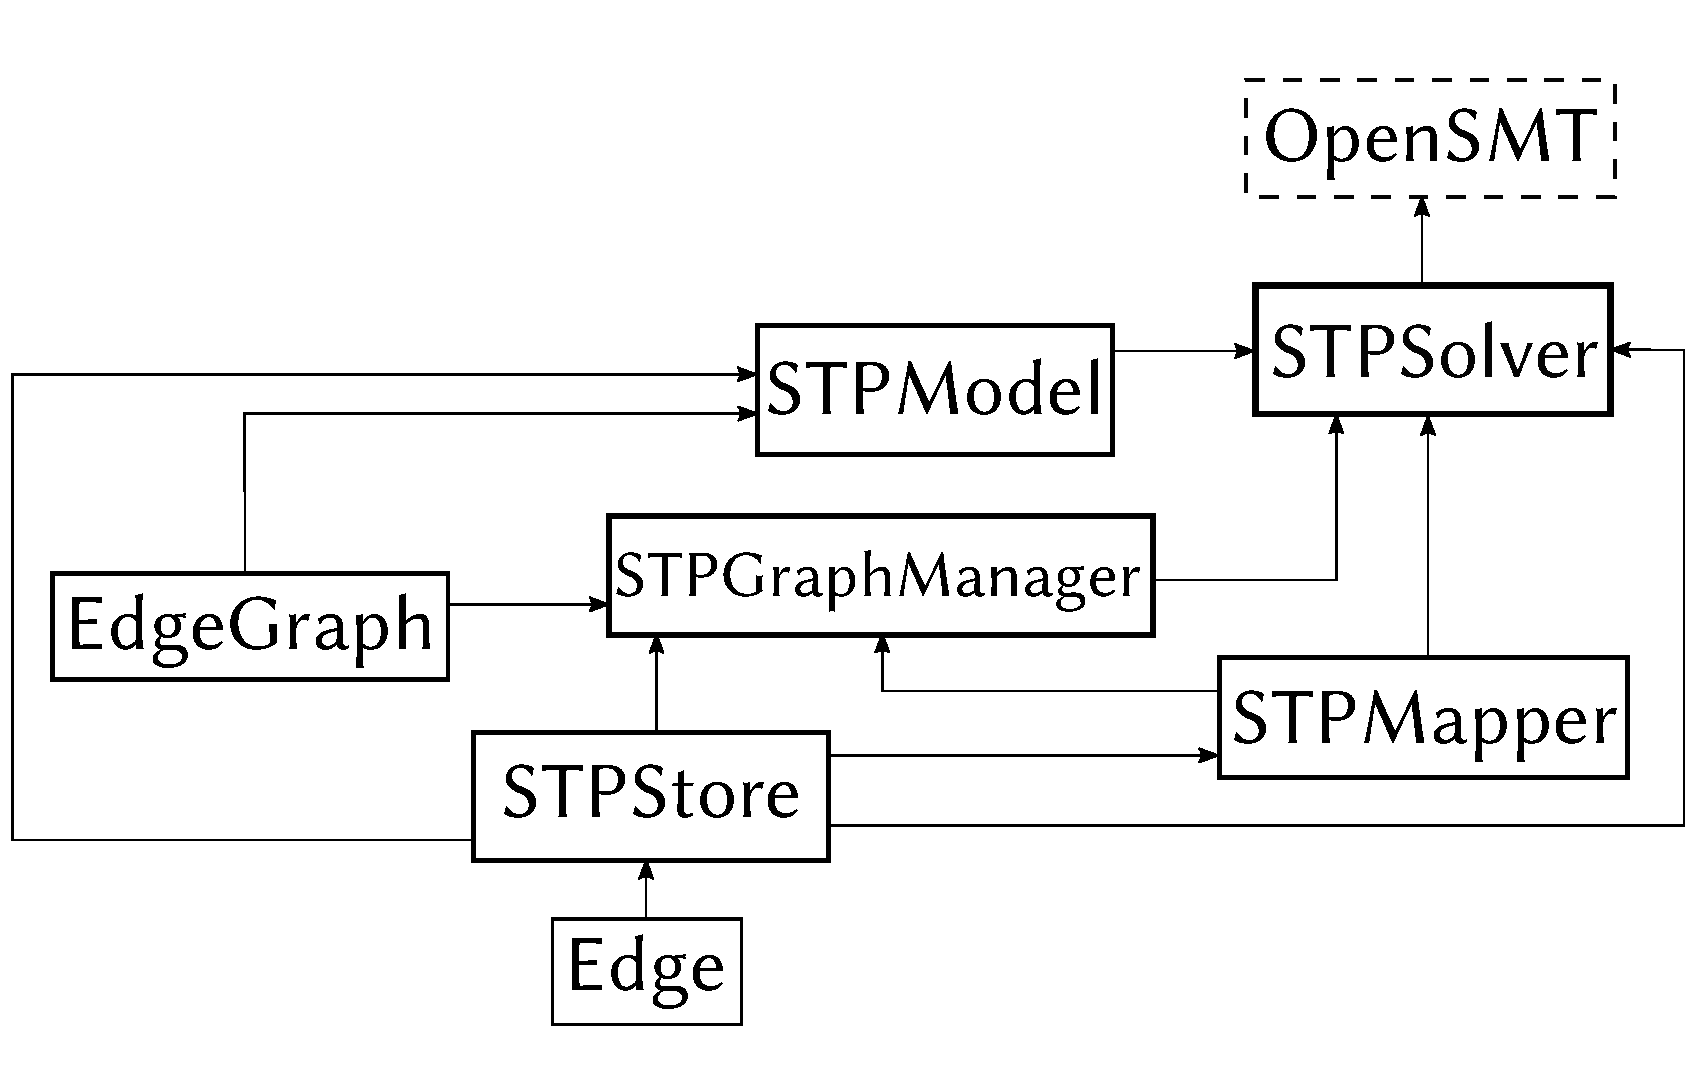
\includegraphics[width=0.8\textwidth]{class_deps}
	\caption{Závislosti mezi strukturami řešiče}
\end{figure}

\section{Přidávání literálů}\label{add}

Na samotném začátku výpočtu se OpenSMT postupně pro každý term zeptá řešiče, zda se jedná o~literál jeho teorie. Jelikož tento proces slouží primárně k~jejich odlišení běžných booleovských termů, nezkoumáme do hloubky struktury termu, ale provádíme jen povrchovou kontrolu. Pokud předpokládáme, že framework použije náš řešič jen pro odpovídající teorii, je taková kontrola dostačující.
\begin{code}
bool STPSolver::isValid(PTRef tr) { return logic.isNumLeq(tr); }
\end{code}

Jakmile jsou termy takto rozlišeny, řešič je informován o~všech literálech, jejichž ohodnocení mu může být oznámeno. K~tomu je využita funkce \icode{declareAtom(PTRef)}. V~té už musíme projít strukturu literálu, abychom z~něj extrahovali relevantní informace. Důležité pro nás přitom je, že díky způsobu, kterým OpenSMT vytváří své termy, nemusíme provádět konverze z~různých tvarů omezení (popsaných v~sekci \ref{stp}). Neostrých nerovností a~obrácených znamének jsme tak v~literálech zbaveni dříve, než se o~nich řešič vůbec dozví --- všechny literály naší teorie jsou reprezentovány standardní formou $c \leq x - y$, popř. $c \leq \pm x$ pro omezení s~jednou proměnnou.\footnote{Tato kanonická transformace mimo jiné ospravedlňuje výše zmíněnou implementaci \icode{isValid}.} Uveďme pro úplnost, že rozdíl je v~této reprezentaci nahrazen součtem záporu. Přesnější popis struktury literálu tak je spíše $c \leq x + (-1 \cdot y)$.

Z~této formy nám už nedělá problém určit hodnotu $c$ a~reference na $x$ a~$y$ postupem naznačeným v~předchozí sekci. Musíme přitom dbát pouze na to, že nerovnice je v~opačné formě než té námi používané. Hrany omezujícího grafu tudíž povedou z~$y$ do $x$ s~ohodnocením $-c$. Tuto odlišnost zdůrazňujeme, protože je v~implementaci práce použití identifikátorů \icode{x} a~\icode{y} standardizováno ve smyslu cílového, resp. zdrojového vrcholu hrany.

\begin{figure}
	\centering
	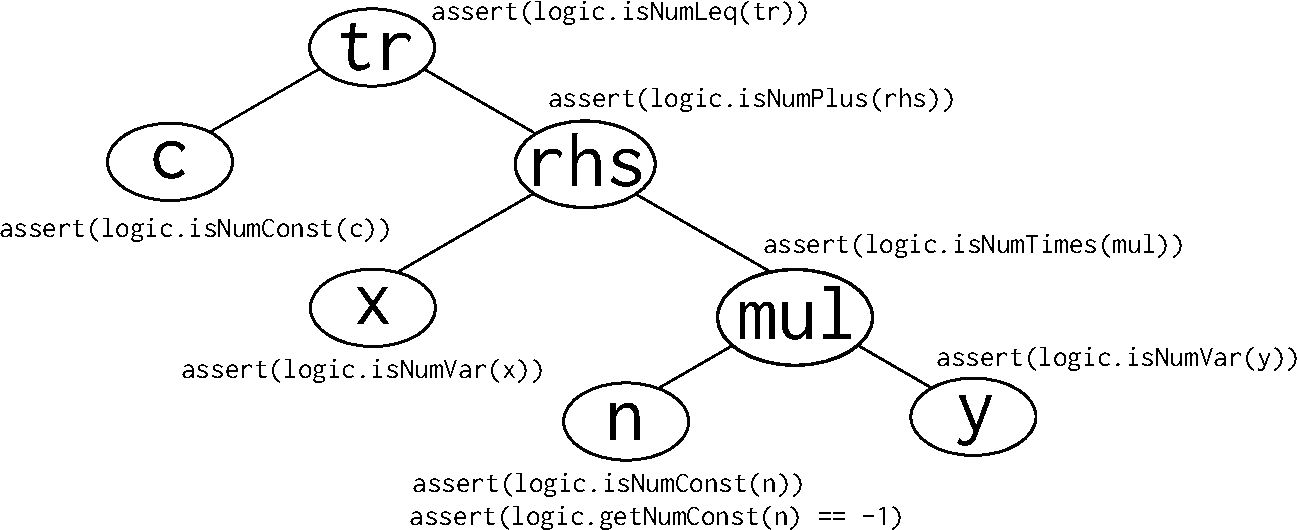
\includegraphics[width=\textwidth]{ptref_structure}
	\caption{Ukázka struktury termu (\icode{PTRef tr} $\approx c \leq x - y$)}
\end{figure}

Jakmile jsme získali informace o~hraně, musíme nejprve zkontrolovat, zda už hrana v~našem řešiči neexistuje. To se může stát, pokud je hrana negací jiné již přidané hrany (viz. níže). %% TODO garbage reference
Hledání hrany probíhá postupným projitím seznamu všech hran, ve kterých se vyskytuje $y$ (seznamy si pro každý vrchol ukládá \icode{STPMapper}). Probíhá tedy lineárně v~počtu hran obsahujících $y$. Jelikož ale přidávání literálů celkově zabírá jen minimální část celého výpočtu, usoudili jsme, že lineární složitost této operace je pro nás přijatelným kompromisem.

Objevíme-li hranu odpovídající přidanému literálu, stačí nám přidat do třídy \icode{STPMapper} tuto asociaci. Všechny ostatní informace o~hraně už známe. V~opačném případě musí ze všeho nejdříve \icode{STPStore} tuto hranu vytvořit (případně s~vrcholy, které jsme ještě nepotkali). Jakmile je hrana vytvořená, vytvoříme předběžně i~její negaci (z~důvodů popsaných v~sekci \ref{upravy}). Obě nově vytvořené hrany pak přidáme do seznamů hran pro jejich vrcholy. U~původní hrany si navíc uložíme její asociaci s~oznámeným literálem (pro negaci zatím tato asociace neexistuje). 

Poté, co tento proces proběhne pro všechny literály ve vstupní formuli, jsme schopni každý literál převézt na odpovídající hranu a~naopak a~dokážeme reprezentovat libovolné ohodnocení přidáním odpovídající hrany do omezujícího grafu.

\section{Oznámení ohodnocení a~hledání důsledků}\label{dusl}

Nejdůležitější část výpočtu se odehrává ve funkci \icode{STPSolver::assertLit}, pomocí které se řešič dozvídá o~nových ohodnocení literálů. Funkce nejprve zkontroluje, zda se řešič nenachází ve sporném stavu. Pokud ano, přidávání další hrany nemá smysl a~funkce okamžitě skončí neúspěchem. V~opačném případě převedeme ohodocení na odpovídající hranu. Následně si uložíme asociaci hrany s~danou proměnnou \icode{PtAsgn}, přidáme ji do omezujícího grafu a~začneme hledat důsledky tohoto přidání. Přidání hrany do grafu znamená její přidání do seznamu hran grafu a~do obou seznamů sousedů a~nastavení její vlastnosti \icode{setTime} na počet aktuálně přidaných hran.

Hledání důsledků zařizuje funkce \icode{STPGraphManager::findConsequences}. Ta nejprve najde seznam možných počátečních a~koncových vrcholů pro cesty procházející přidanou hranou. K~tomu využíváme prohledávání do hloubky, jak bylo popsané v~referenčním algoritmu. Prohledávání přitom probíhá sekvenčně --- nejprve hledáme počáteční vrcholy, poté hledáme vrcholy cílové. Jelikož prohledávání na společných datech provádí pouze čtecí operace, bylo by možné tento proces paralelizovat a~hledat obě množiny současně. Během vývoje jsme zkoušeli uplatnit tento přístup, nicméně režie vytváření a~rušení vláken  se ukázala časově náročnější než samotné prohledávání. Prozkoumali jsme také možnost nastavit hranici na velikost grafu určující, zda výpočet proběhne sekvenčně, či paralelně. V~praxi se ale ukázalo, že hranice byla buď příliš vysoká a~vícevláknový přístup nebyl nikdy použit, nebo byla příliš nízká a~použití vláken stále zhoršovalo výkonnost programu. Rozhodli jsme se tak zůstat u~běžné jednovláknové varianty. Využití perzistentního pole vláken nebo rigoróznější hledání limitu pro použití vlákna jsou možné oblasti dalšího zkoumání, dle našeho úsudku by ale nepřinesly podstatné zrychlení algoritmu.

Poté, co obě množiny nalezneme, vybereme tu, jejíž vrcholy se celkově objevují v~menším množství hran (tyto součty počítáme v~průběhu DFS). Pro kažý vrchol z~vybrané množiny projdeme seznam všech hran, v~nichž se vyskytuje (tyto seznamy si ukládá \icode{STPMapper}) a~uložíme si všechny, které jsou důsledky naposledy přidané hrany. Aby byla hrana $a \xrightarrow{c'} b$ důsledkem právě přidané hrany $y \xrightarrow{c} x$, musí platit 
\begin{enumerate}
	\item Existuje cesta $a \rightarrow y \xrightarrow{c} x \rightarrow b$.
	\item $c'$ je větší než délka nekratší takové cesty.
\end{enumerate}

Snadno nahlédneme, že tyto dvě podmínky pokrývají právě všechna omezení, která jsou důsledky přidání hrany $y \xrightarrow{c} x$ do grafu. Jakmile objevíme všechny takovéto hrany, musíme je převézt zpět do tvaru \icode{PtAsgn} a~předat je frameworku. Odpovídá-li přitom hraně \icode{h} literál \icode{tr} a~negaci \icode{h} literál \icode{nr}, objevení \icode{h} jakožto důsledku způsobí označení \icode{PtAsgn(tr,true)} a~\icode{PtAsgn(nr,false)} jako důsledků oznámeného ohodnocení (pokud \icode{tr} a~\icode{nr} existuje). Pokud existuje odpovídající literál \icode{nr} i~k~negaci hrany právě přidané do grafu, nesmíme zapomenout ani na vytvoření důsledku \icode{PtAsgn(nr,false)} pro tuto hranu.

Oznamování takto nalezených dedukcí provádíme pomocí rozhraní abstraktní třídy \icode{TSolver}, jíž je \icode{STPSolver} potomkem. Ta poskytuje funkci \icode{storeDeduction}, které můžeme předat námi vytvořené důsledky. Funkce technicky vzato bere jako parametr strukturu \icode{PtAsgn\_reason}, jež ale v~řešiči existuje pouze z~historických důvodů a~funkčně se nijak neliší od běžného \icode{PtAsgn}. Voláním \icode{storeDeduction} uložíme nalezené důsledky ve vnitřní struktuře \icode{TSolver}, z~níž už je zbytek řešiče dokáže získat.

\section{Rozhodování o~splnitelnosti}\label{rozhod}

Jak už jsme naznačili v~sekci \ref{upravy}, samotné rozhodování o~splnitelnosti současného ohodnocení (implementované funkcí \icode{STPSolver::check}) je v~podstatě prázdnou operací. To je důsledkem využití vyčerpávající propagace teorie. Je-li některé možné ohodnocení sporné s~aktuálním omezujícím grafem, museli jsme objevit hranu odpovídající takovému ohodnocení jako důsledek tohoto grafu. K~detekování sporného ohodnocení nám tak stačí zkontrolovat přítomnost této negace ve chvíli, kdy je nám ohodnocení oznámeno.

Kontrolu proto provádíme ve funkci \icode{STPSolver::assertLit}. Ihned poté, co převedeme ohodnocený literál na odpovídající hranu (jak popisuje předchozí sekce), zjistíme, zda je \emph{pravdivá} negace hrany (je součástí omezujícího grafu nebo jeho nalezeným důsledkem). Pokud ano, řešič přejde do sporného stavu a~okamžitě frameworku oznámí neúspěšné ohodnocení. Pokud ne, funkce může pokračovat s~jistotou, že ohodnocení není sporné a~nevytvoří v~grafu žádný záporný cyklus. Pravdivost hrany v~této kontrole určujeme podle její vlastnosti \icode{Edge::setTime}, která je právě u~pravdivých hran nenulová.

Současný stav řešiče indikuje proměnná \icode{STPSolver::inv\_asgn}. Ve sporném stavu proměnná ukládá ohodnocení, kterým se do sporného stavu dostala. V~konzistentním stavu obsahuje výchozí hodnotu \icode{PtAsgn\_Undef}, reprezentující absenci takového ohodnocení. Když přecházíme do sporného stavu, zapamatujeme si navíc v~proměnné \icode{STPSolver::inv\_bpoint} záchytný bod, ve kterém se řešič právě nachází. Tyto hodnoty jsou pro nás důležité pro mechanismus hledání konfliktů a~správné vyhodnocení backtrackingu. Samotnou funkci \icode{check} pak můžeme implementovat jako jednoduchou kontrolu proměnné \icode{inv\_asgn}.

\begin{code}
TRes STPSolver::check(bool b) { 
	return inv_asgn == PtAsgn_Undef ? TRes::SAT : TRes::UNSAT; 
}
\end{code}
Pro úplnost dodejme, že parameter \icode{b} v~signatuře funkce \icode{check} určuje, zda se jedná pouze o~přechodnou kontrolu probíhající v~průběhu výpočtu, nebo závěrečnou kontrolu provedenou až na jeho samotném konci. Jelikož náš přístup tyto varianty nerozlišuje, můžeme hodnotu parametru ignorovat.

\section{Hledání konfliktů a~backtracking}

Poté, co řešič oznámí sporný stav, se od něj zpravidla vyžaduje, aby detekoval množinu ohodnocení, jež tento stav způsobují. Množina by přitom měla být pokud možno co nejmenší --- jednoduché vrácení všech dosavadních ohodnocení je sice korektní, ale pro účely SMT řešiče naprosto zbytečné. Řešiče v~OpenSMT za tímto účelem musí implementovat funkci \icode{getConflict}.

Náš řešič konliktní množinu hledá pomocí operace \icode{Explain} popsané v~referenčním algoritmu. Tuto operaci provádí funce \icode{STPGraphManager::findExplanation}. K~určení hrany \icode{h}, jejíž vysvětlení hledáme, nám slouží proměnná \icode{inv\_asgn}. Ze třídy \icode{STPMapper} nejprve získáme hranu odpovídající hodnotě \icode{inv\_asgn}. Konfliktní množina je pak ekvivalentní vysvětlení negace této hrany. 

\begin{code}
void STPSolver::getConflict(vec<PtAsgn> &v) {
	EdgeRef e = mapper.getEdgeRef(inv_asgn.tr);
	if (inv_asgn.sgn == l_True)
	    e = store.getNegation(e);
	
	graphMgr.findExplanation(e, v);
	v.push(inv_asgn);
}
\end{code}

Hledání vysvětlení provádí \icode{STPGraphManager} modifikovanou verzí DFS, která probíhá podobně jako při hledání důsledků, ovšem s~několika malými změnami. Začínáme v~počátečním vrcholu \icode{h}. Z~něj spustíme prohledávání popsané v~sekci \ref{dusl}, ve kterém si navíc pro každý vrchol pamatujeme, ze kterého vrcholu byl naposledy navštíven. Prohledávání také prochází pouze přes hrany, které nemají \icode{setTime} vyšší než \icode{h} (čímž zajišťujeme, že se ve vysvětlení neobjevují hrany přidané až po \icode{h}), a~navštěvuje pouze vrcholy, jejichž vzdálenost není vyšší než cena \icode{h} (čímž proces zrychlujeme).

Vzhledem k~podobnostem s~hledáním důsledků jsme zvažovali pouze rozšíření existující funkce \icode{STPGraphManager::dfsSearch} k~tomuto účelu. Drobné rozdíly mezi oběma postupy ale jejich integraci do společné funkce nakonec zabránily. Pokrytí všech možností průběhu v~obou případech by znamenalo zhoršení čitelnosti kódu a~pravděpodobně by se podepsalo i~na rychlosti operace. Rozhodli jsme se proto implementovat \icode{findExplanation} jako samostatnou funkci.

Jakmile DFS skonční, projdeme v~uloženém seznamu předchůdců zpětně cestu z~cílového do zdrojového vrcholu. Hrany této cesty můžeme označit jako příčiny \icode{h}. Tyto hrany je nakonec třeba převést na jejich odpovídající \icode{PtAsgn} proměnné. Převodů jsme zaručeně schopni, neboť omezující graf obsahuje pouze explicitně ohodnocené hrany a~nikoliv nalezené důsledky. Aby se nakonec z~množiny příčin stala konfliktní množina, stačí nám do ní přidat \icode{inv\_asgn}, čímž uzavřeme záporný cyklus v~grafu. 

Speciální případ problému nastává ve chvíli, kdy \icode{h} odpovídá některému oznámenému ohodnocení, tedy je sama součástí grafu. V~takovém případě nemusí hledání vůbec probíhat. Konfliktní množina je totiž triviálně \{\icode{h}, \icode{$\neg$h}\}, respektive jejich odpovídající hodnoty \icode{PtAsgn}.

Vrácenou množinu framework analyzuje a~rozhodne podle ní o~dostatečné úrovni backtrackingu. Ten probíhá na bázi záchytných bodů. OpenSMT může kdykoliv zavolat na řešiči funkci \icode{pushBacktrackPoint} a~řešič si musí zapamatovat svůj aktuální stav. V~budoucnu pak může framework použitím funkce \icode{popBacktrackPoint} vrátit řešič do stavu těsně před posledním zavoláním \icode{pushBacktrackPoint}. Existuje i~obecnější varianta funkce zvaná \icode{popBacktrackPoints}, která jako parametr přijímá počet záchytných bodů, jež má řešič \uv{zahodit}.

Pro implementaci tohoto systému v~našem řešiči si uvědomme, že v~záchytných bodech nám stačí pamatovat si aktuální stav omezujícího grafu a~aktuální převody mezi ohodnoceními a~hranami. Hodnoty v~\icode{STPStore} ani převody z~\icode{PTRef} na \icode{EdgeRef} se totiž mezi záchytnými body nemohou měnit.

\begin{code}
void STPSolver::pushBacktrackPoint() {
	TSolver::pushBacktrackPoint();
	backtrack_points.push(graphMgr.getAddedCount());
}
\end{code}

Jelikož si navíc ukládáme přidané hrany v~grafu chronologicky do seznamu, stačí nám ve skutečnosti k~jednoznačnému určení záchytného bodu jen současný počet přidaných hran. Jakmile ho máme, můžeme při návratu postupně odebírat hrany z~konce seznamu. Každou odebranou hranu pak odstraníme i~z~odpovídajících seznamů sousedů (ty jsou rovněž chronologické, odebíraná hrana je tudíž na jejich konci), vynulujeme její \icode{setTime} a~odstraníme její asociaci s~hodnotou \icode{PtAsgn}. Ze seznamu dedukcí také musíme odstranit všechny dedukce, které mají \icode{setTime} vyšší nebo roven odebírané hraně.  Tyto operace má na starost funkce \icode{STPGraphManager::removeAfter}. 

Jak snadno nahlédneme z~předchozího odstavce, celý proces probíhá v~lineárním čase vzhledem k~počtu odebíraných hran. Byl-li navíc před návratem řešič ve sporném stavu, zkontrolujeme nakonec hodnotu proměnné \icode{inv\_bpoint}. Pokud se backtrackingem vracíme až před záchytný bod uložený v~této proměnné, můžeme řešič vrátit zpět do konzistentního stavu.

\section{Nalezení splňujícího ohodnocení}

Pokud o~nějaké formuli rozhodneme, že je splnitelná, může být zajímavé najít nějaké její splňující ohodnocení. Pro řešič teorie to znamená najít splňující ohodnocení jemu předané konjunkce literálů. Za tímto účelem v~našem řešiči vznikla třída \icode{STPModel}, která vytváří a~ukládá ohodnocení vrcholů omezujícího grafu. Instanci třídy předáme kopii grafu jako parametr. Následně využijeme její funkce \icode{computeModel}, která sestrojí mapu určující ohodnocení vrcholů následujícím způsobem.

Nejprve přidáme do grafu nový vrchol a~propojí ho přes nulové hrany se všemi ostatními vrcholy. Následně spustíme hledání nejkratší cesty z~tohoto nově přidaného vrcholu do všech ostatních vrcholů. Jelikož model hledáme pouze ve splnitelných ohodnoceních, graf zaručeně neobsahuje záporné cykly a~délka nejkratší cesty je pro každý vrchol dobře definovaná. Cesty hledáme klasickým Bellman-Fordovým algoritmem, po jehož skončení si nalezené délky uložíme do mapy. Na závěr zkontrolujeme, zda se v~grafu nevyskytuje vrchol symbolizující proměnnou $zero$ (viz.~sekce \ref{stp}). Pokud ano, všechny hodnoty v~mapě posuneme tak, aby vrchol $zero$ měl nulové ohodnocení.
\begin{code}
void STPModel::computeModel() {
	VertexRef start = addStartingPoint();
	bellmanFord(start);
	shiftZero();
}
\end{code}
Není těžké ukázat, že vezmeme-li negace nalezených délek, dostaneme splňující ohodnocení vrcholů. Z~tvrzení \ref{tvr:posun} pak vyplývá, že závěrečný posun nám splnitelnost nerozbije.

Jelikož instanci \icode{STPModel} potřebujeme vždy nejvýše jednu, navíc ji potřebujeme vytvořit až na samotný závěr výpočtu, ukládáme si ji pouze ve formě ukazatele (který má v~průběhu výpočtu hodnotu \icode{nullptr}). Protože navíc přístup k~tomuto ukazateli potřebuje pouze třída \icode{STPSolver}, využíváme chytrý ukazatel typu \icode{std::unique\_ptr}.

Komunikace se zbytkem frameworku pak probíhá ve dvou krocích. Nejprve je zavolána funkce \icode{STPSolver::computeModel}. Ta vytvoří model teorie tak, jak bylo popsáno výše. Následuje opakované volání funkce \icode{STPSolver::getValue}, kde řešič vrací frameworku hodnoty jednotlivých literálů teorie, pokud je zná. V~době psaní této práce bohužel existuje chyba v~implementaci \icode{getValue} způsobující, že v~okrajových případech není řešič schopen správně odpovědět na některé dotazy frameworku. Mimo tyto výjimečné situace však dle našeho testování funguje tvorba modelu korektně.
%% TODO remove disclaimer if we fix it in time
